\documentclass[../231120_msquare_computational-logic.tex]{subfiles}
\begin{document}

\begin{frame}{So far...}
    이때까지 한 것:
    \begin{center}
        \fbox{
            \begin{minipage}{.9\textwidth}
                \begin{itemize}
                    \ii Signature \((\mcal F, \mcal R, \mrm{ar})\) 넣어서
                        FOL Language \(\mcal L\) 만들기
                    \ii \(\Lang\)에 \(\Lang\)-structure \(\mcal M = (U, \mcal I)\)으로 의미를 부여하기
                \end{itemize}
            \end{minipage}
        }
    \end{center}
    \pause
    \begin{alertblock}{}
        이제부터 할 것:
        \begin{itemize}
            \ii \(S \vDash A\)인지 확인할 방법 찾으려고 시도...
                \begin{itemize}
                    \ii \(S \vDash A\)와 equivalent한 좋은 명제 없을까?
                    % \ii 이왕이면 computable한 방법(proof theory)으로.
                    % \ii 여기서 computable: 대충 `컴퓨터가 할 수 있음'으로 이해
                \end{itemize}
        \end{itemize}
    \end{alertblock}
\end{frame}

\subsection{Proof}
\begin{frame}{Sequent}
    \begin{alertblock}{들어가기에 앞서}
        Proof theory는 semantics와 전혀 관련이 없음.
        둘의 연관성은 나중에 볼 예정.
    \end{alertblock}
    \pause
    \begin{block}{Definition: Sequent \(\Gamma \vdash A\)}
        A sequent is a pair \((\Gamma, A)\) where \(\Gamma \subseteq \Lang\) and \(A \in \Lang\).
        (보통 \alert{\(\Gamma \vdash A\)}로 씀.)
    \end{block}
    \(\Gamma\)는 공리(axiom), \(A\)는 결론(conclusion)이라고 보면 됨.

    % \begin{exampleblock}{Example}
    %     \begin{itemize}
    %         \ii \((\text{Peano axioms}) \vdash (x \le y \land x \neq y \ \Rightarrow\ S(x) \le y)\)
    %     \end{itemize}
    % \end{exampleblock}
\end{frame}

\begin{frame}{Proof on Sequent (Gentzen-style)}
    \begin{block}{Definition: Proof on Sequents}
        A \alert{proof} of a sequent \(\Gamma \vdash A\) is a \alert{tree} such that
        \begin{itemize}
            \ii its root is the sequent \(\Gamma \vdash A\) and
            \ii its \alert{subtrees are proofs} of sequents \(\Gamma_1 \vdash A_1, \cdots, \Gamma_k \vdash A_k\) where
                \begin{prooftree}
                \AxiomC{\(\Gamma_1 \vdash A_1\)}
                \AxiomC{\(\Gamma_2 \vdash A_2\)}
                \AxiomC{\(\cdots\)}
                \AxiomC{\(\Gamma_k \vdash A_k\)}
                \QuaternaryInfC{\(\Gamma \vdash A\)}
                \end{prooftree}
                is a \fbox{natural deduction}.
        \end{itemize}
        If \(\Gamma \vdash A\) has a proof, then we say \(\Gamma \vdash A\) is \alert{provable}.
    \end{block}
    \pause

    \begin{exampleblock}{}
        \begin{itemize}
            \ii Natural deduction은 가장 작은 단위의 reasoning
                \begin{itemize}
                    \ii 뒤에서 볼 예정
                \end{itemize}
            \ii \(\Gamma \vdash A\): 증명하고자 하는 것
            \ii \(\Gamma_1 \vdash A_1, \cdots, \Gamma_k \vdash A_k\): \(\Gamma \vdash A\)의 \ul{근거}
        \end{itemize}
    \end{exampleblock}
\end{frame}

\begin{frame}{Natural Deduction}
    얘네들이 natural deduction (겁먹을 필요 없음): \vspace*{-1.7em}
    \begin{columns}
    \begin{column}{0.27\textwidth}
        \begin{center}
        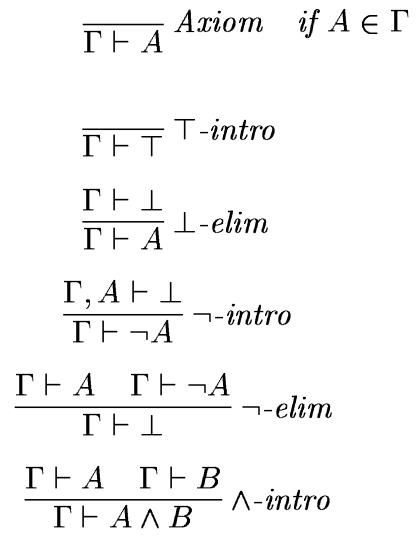
\includegraphics[width=1.2\textwidth]{./natural_deduction_1.png}
        \end{center}
    \end{column}
    \begin{column}{0.3\textwidth}
        \begin{center}
        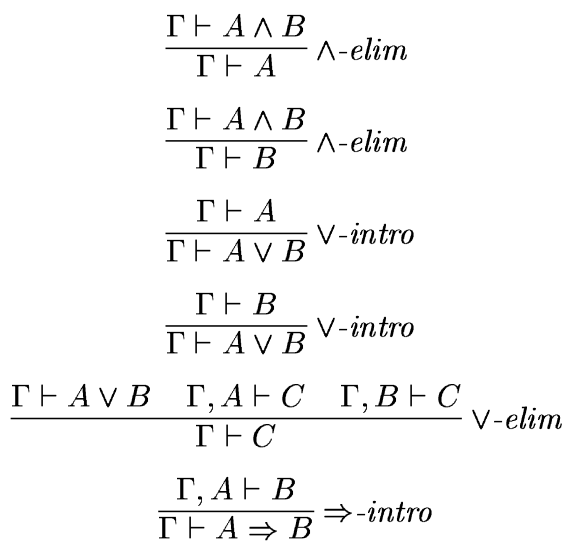
\includegraphics[width=1.2\textwidth]{./natural_deduction_2.png}
        \end{center}
    \end{column}
    \begin{column}{0.3\textwidth}
        \begin{center}
        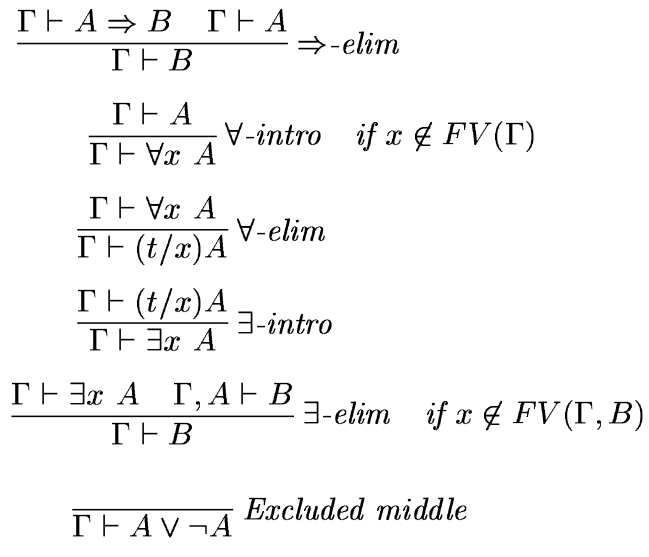
\includegraphics[width=1.1\textwidth]{./natural_deduction_3.png}
        \end{center}
    \end{column}
    \end{columns}
    \pause

    \begin{alertblock}{}
        \begin{itemize}
            \ii 가로선 위에서부터 아래로 deduction이 일어남.
                \begin{itemize}
                    \ii 위의 sequent들이 provable하면 아래도 provable
                \end{itemize}
            \ii 이름이 natural deduction인 만큼 하나씩 뜯어보면 당연함.
                \begin{itemize}
                    \ii 직관을 글로 explicit하게 쓰려고 하니 벌어지는 참사...
                \end{itemize}
        \end{itemize}
    \end{alertblock} 
\end{frame}

\begin{frame}{Formal Proof: Example}
    \begin{exampleblock}{}
        \(\Gamma, A\vdash C\)는 \(\Gamma \cup \{A\} \vdash C\)의 shortcut
    \end{exampleblock}
    Proof of \(\Gamma \vdash A \Rightarrow (B \Rightarrow (A \land B))\):
    \begin{prooftree}
        \AxiomC{}
        \RightLabel{\small Axiom}
        \UnaryInfC{\(\Gamma, A, B \vdash A\)}
                \AxiomC{}
                \RightLabel{\small Axiom}
                \UnaryInfC{\(\Gamma, A, B \vdash B\)}
                \RightLabel{\small \(\land\)-intro}
            \BinaryInfC{\(\Gamma, A, B \vdash A \land B\)}
            \RightLabel{\small \(\Rightarrow\)-intro}
            \UnaryInfC{\(\Gamma, A\vdash B \Rightarrow (A \land B)\)}
            \RightLabel{\small \(\Rightarrow\)-intro}
            \UnaryInfC{\(\Gamma\vdash A \Rightarrow (B \Rightarrow (A \land B))\)}
    \end{prooftree}

    Reference:
    \begin{center}
        \fbox{
            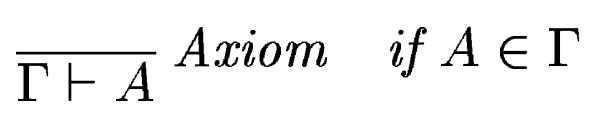
\includegraphics[width=.25\textwidth]{./nat_axiom.png}
        }
        \fbox{
            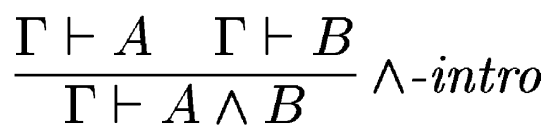
\includegraphics[width=.25\textwidth]{./nat_and_intro.png}
        }
        \fbox{
            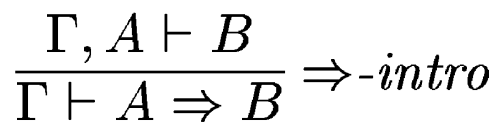
\includegraphics[width=.25\textwidth]{./nat_implies_intro.png}
        }
    \end{center}
\end{frame}

\begin{frame}{Soundness of FOL}
    \begin{block}{Theorem (Soundness of FOL)}
        For every \(\Gamma \subseteq \LS\) and \(A \in \LS\),
        \centerline{\(\Gamma \vdash A \text{ is provable} \ \implies\ \Gamma \vDash A\).}
    \end{block}
    \begin{block}{Proof}
        Natural induction을 이 theorem이 성립하도록 잡았기 때문...
        엄밀한 증명은 정말 귀찮음. \qed
    \end{block}
    \begin{exampleblock}{Recall: Logical Consequence}
        If \(\mcal M \vDash S \ \implies\ \mcal M \vDash A\) for every \(\Lang\)-structure \(\mcal M\),
        we say \(A\) is a \ul{logical consequence} of \(S\)
        and we write \(S \vDash A\).
    \end{exampleblock}

    \begin{alertblock}{}
        \centerline{증명의 존재는 진리치가 참임을 함의함!}
    \end{alertblock}
\end{frame}

\begin{frame}{Completeness of FOL}
    \begin{block}{Theorem (Completeness of FOL) \hfill [Gödel, 1929]}
        For every \(\Gamma \subseteq \LS\) and \(A \in \LS\),
        \centerline{\(\Gamma \vDash A\ \implies\ \Gamma \vdash A \text{ is provable} \).}
    \end{block}
    \begin{block}{Proof}
        \pause
        ...를 여기서 하면 세미나 \(n\)시간 추가됨.
        \begin{itemize}
            \ii 1929년 괴델의 증명보다 1949년 Henkin의 증명이 더 쉽고 짧음.
        \end{itemize}
    \end{block}
    \begin{alertblock}{}
        아니 Gödel의 First Incompleteness Theorem에 의하면
        ZFC에 증명도 반증도 할 수 없는 명제가 있는데 어떻게 된 것? \pause
        \begin{itemize}
            \ii 위 theorem은 \(\Gamma\)의 모든 model이 \(A\)의 model이기도 하다는 것
            \ii 증명도 반증도 할 수 없는 명제 \(A\)와 \(\lnot A\) 둘 다 \(\Gamma\)의 logical consequence가 아님!
        \end{itemize}
    \end{alertblock}
\end{frame}

\subsection{Automatic Theorem Verification / Theorem Proving}

\begin{frame}{Automatic Proof Verification}
    우리는 방금:
    \begin{center}
        \fbox{Proof를 computable object(tree)로 formalize함}
    \end{center}
    \begin{exampleblock}{Proof tree의 특징}
        \begin{enumerate}
            \ii 모든 Proof Tree의 set은 countable.
                \begin{itemize}
                    \ii Natural deduction의 개수가 finite
                    \ii 한 번에 늘어나는 subtree의 개수가 finite
                    \ii 모든 proof tree의 height는 finite
                \end{itemize}
            \ii 어느 proof tree가 valid한지 \ul{쉽게} 확인 가능
                \begin{itemize}
                    \ii finite 개수의 natural deduction => finite 횟수의 확인
                \end{itemize}
        \end{enumerate}
    \end{exampleblock}
\end{frame}

\begin{frame}{Automatic Theorem Proving}
    \begin{exampleblock}{Theorem에서 proof 찾기}
        \(\Gamma \subseteq \LS, A \in \LS\)
        \begin{enumerate}
            \ii 모든 Proof Tree를 열거하면서:
            \ii 그 tree \(T\) 가 \(\Gamma \vdash A\)인지 확인
            \ii 맞으면 \(T\)가 그 증명. 아니면 계속 진행...
        \end{enumerate}
    \end{exampleblock}
    \pause

    \begin{exampleblock}{모든 Theorem 찾기}
        \begin{enumerate}
            \ii 모든 \(A \in \LS\)와 \(\Gamma \vdash A\)를 root로 가지는 모든 Proof Tree를 열거하면서:
            \ii 그 tree \(T\) 가 \(\Gamma \vdash A\)인지 확인
            \ii 맞으면 \(A\)는 theorem. 아니면 계속 진행...
        \end{enumerate} 
        \pause
        만약 이게 가능하다면, 수학자들이 실직하지 않는 이유는 단순히 computing power의 부족 때문...
    \end{exampleblock}
\end{frame}

\begin{frame}{Automatic Theorem Proving : Example}
    \begin{exampleblock}{\textsc{Coq}}
        Computer software의 하나:
        \begin{itemize}
            \ii Proof tree를 쉽게(?) 구성할 수 있도록 해 줌.
            \ii 엄청난 표현력...
            \ii 부분적 \ul{automated theorem proving}
            \ii Cryptography 분야에서는 Coq proof 증명을 요구하기도...
        \end{itemize}
    \end{exampleblock}

    \begin{exampleblock}{\textsc{Coq} Proof of \(\sum_{i=1}^{n} (2n^3+3n^2+n)/6\)}
        \small
        \ttt{%
Lemma sum3: forall n:nat, 6*sum n = 2*n*n*n + 3*n*n + n. \\
Proof. \\
\ \ \ \ induction n. \\
\ \ \ \ simpl (sum 0). ring; simpl (sum (S n)). \\
\ \ \ \ ring simplify; rewrite IHn. \\
\ \ \ \ ring. \\
Qed.}
    \end{exampleblock}
\end{frame}

\end{document}
